%File: anonymous-submission-latex-2026.tex
\documentclass[letterpaper]{article} % DO NOT CHANGE THIS
\usepackage[submission]{aaai2026}  % DO NOT CHANGE THIS
\usepackage{times}  % DO NOT CHANGE THIS
\usepackage{helvet}  % DO NOT CHANGE THIS
\usepackage{courier}  % DO NOT CHANGE THIS
\usepackage[hyphens]{url}  % DO NOT CHANGE THIS
\usepackage{graphicx} % DO NOT CHANGE THIS
\urlstyle{rm} % DO NOT CHANGE THIS
\def\UrlFont{\rm}  % DO NOT CHANGE THIS
\usepackage{natbib}  % DO NOT CHANGE THIS AND DO NOT ADD ANY OPTIONS TO IT
\usepackage{caption} % DO NOT CHANGE THIS AND DO NOT ADD ANY OPTIONS TO IT
\frenchspacing  % DO NOT CHANGE THIS
\setlength{\pdfpagewidth}{8.5in} % DO NOT CHANGE THIS
\setlength{\pdfpageheight}{11in} % DO NOT CHANGE THIS
%
% These are recommended to typeset algorithms but not required. See the subsubsection on algorithms. Remove them if you don't have algorithms in your paper.
\usepackage{algorithm}
\usepackage{algorithmic}
\usepackage{amsmath}
\usepackage{amssymb}
\usepackage{bm}

%
% These are are recommended to typeset listings but not required. See the subsubsection on listing. Remove this block if you don't have listings in your paper.
\usepackage{newfloat}
\usepackage{listings}
\DeclareCaptionStyle{ruled}{labelfont=normalfont,labelsep=colon,strut=off} % DO NOT CHANGE THIS
\lstset{%
	basicstyle={\footnotesize\ttfamily},% footnotesize acceptable for monospace
	numbers=left,numberstyle=\footnotesize,xleftmargin=2em,% show line numbers, remove this entire line if you don't want the numbers.
	aboveskip=0pt,belowskip=0pt,%
	showstringspaces=false,tabsize=2,breaklines=true}
\floatstyle{ruled}
\newfloat{listing}{tb}{lst}{}
\floatname{listing}{Listing}
%
% Keep the \pdfinfo as shown here. There's no need
% for you to add the /Title and /Author tags.
\pdfinfo{
/TemplateVersion (2026.1)
}

% DISALLOWED PACKAGES
% \usepackage{authblk} -- This package is specifically forbidden
% \usepackage{balance} -- This package is specifically forbidden
% \usepackage{color (if used in text)
% \usepackage{CJK} -- This package is specifically forbidden
% \usepackage{float} -- This package is specifically forbidden
% \usepackage{flushend} -- This package is specifically forbidden
% \usepackage{fontenc} -- This package is specifically forbidden
% \usepackage{fullpage} -- This package is specifically forbidden
% \usepackage{geometry} -- This package is specifically forbidden
% \usepackage{grffile} -- This package is specifically forbidden
% \usepackage{hyperref} -- This package is specifically forbidden
% \usepackage{navigator} -- This package is specifically forbidden
% (or any other package that embeds links such as navigator or hyperref)
% \indentfirst} -- This package is specifically forbidden
% \layout} -- This package is specifically forbidden
% \multicol} -- This package is specifically forbidden
% \nameref} -- This package is specifically forbidden
% \usepackage{savetrees} -- This package is specifically forbidden
% \usepackage{setspace} -- This package is specifically forbidden
% \usepackage{stfloats} -- This package is specifically forbidden
% \usepackage{tabu} -- This package is specifically forbidden
% \usepackage{titlesec} -- This package is specifically forbidden
% \usepackage{tocbibind} -- This package is specifically forbidden
% \usepackage{ulem} -- This package is specifically forbidden
% \usepackage{wrapfig} -- This package is specifically forbidden
% DISALLOWED COMMANDS
% \nocopyright -- Your paper will not be published if you use this command
% \addtolength -- This command may not be used
% \balance -- This command may not be used
% \baselinestretch -- Your paper will not be published if you use this command
% \clearpage -- No page breaks of any kind may be used for the final version of your paper
% \columnsep -- This command may not be used
% \newpage -- No page breaks of any kind may be used for the final version of your paper
% \pagebreak -- No page breaks of any kind may be used for the final version of your paperr
% \pagestyle -- This command may not be used
% \tiny -- This is not an acceptable font size.
% \vspace{- -- No negative value may be used in proximity of a caption, figure, table, section, subsection, subsubsection, or reference
% \vskip{- -- No negative value may be used to alter spacing above or below a caption, figure, table, section, subsection, subsubsection, or reference

\setcounter{secnumdepth}{0} %May be changed to 1 or 2 if section numbers are desired.

% Custom macros
\newcommand{\bxi}{\boldsymbol{\xi}}
\newcommand{\bx}{\bm{x}}
\newcommand{\avg}[1]{\langle #1 \rangle}
\newcommand{\e}{{\mathrm{e}}}
\newcommand{\dd}{{\mathrm{d}}}
% \newcommand{\Bnet}{\beta_{\mathrm{net}}}
\newcommand{\Bnet}{\beta}
\newcommand{\phieq}{\phi_{\mathrm{eq}}}
\newcommand{\fret}{f_{\mathrm{ret}}}
\newcommand{\gmax}{g_{\max}}
\newcommand{\acGauss}{\alpha_c^{\mathrm{G}}}
\newcommand{\acBd}{\alpha_c^{\mathrm{bd}}}
\newcommand{\acSd}{\alpha_c^{\mathrm{sd}}}
\newcommand{\acSp}{\alpha_c^{\mathrm{sp}}}
\newcommand{\p}{\partial}
\newcommand{\cas}{\textstyle\frac}


% The file aaai2026.sty is the style file for AAAI Press
% proceedings, working notes, and technical reports.
%

% Title

% Your title must be in mixed case, not sentence case.
% That means all verbs (including short verbs like be, is, using,and go),
% nouns, adverbs, adjectives should be capitalized, including both words in hyphenated terms, while
% articles, conjunctions, and prepositions are lower case unless they
% directly follow a colon or long dash
\title{\bfseries Thermodynamic approach and Saddle-Dominated Capacity
of the LSE Dense Associative Memory}

\author{
    %Authors
    % All authors must be in the same font size and format.
    Written by AAAI Press Staff\textsuperscript{\rm 1}\thanks{With help from the AAAI Publications Committee.}\\
    AAAI Style Contributions by Pater Patel Schneider,
    Sunil Issar,\\
    J. Scott Penberthy,
    George Ferguson,
    Hans Guesgen,
    Francisco Cruz\equalcontrib,
    Marc Pujol-Gonzalez\equalcontrib
}
\affiliations{
    %Afiliations
    \textsuperscript{\rm 1}Association for the Advancement of Artificial Intelligence\\
    % If you have multiple authors and multiple affiliations
    % use superscripts in text and roman font to identify them.
    % For example,

    % Sunil Issar\textsuperscript{\rm 2},
    % J. Scott Penberthy\textsuperscript{\rm 3},
    % George Ferguson\textsuperscript{\rm 4},
    % Hans Guesgen\textsuperscript{\rm 5}
    % Note that the comma should be placed after the superscript

    1101 Pennsylvania Ave, NW Suite 300\\
    Washington, DC 20004 USA\\
    % email address must be in roman text type, not monospace or sans serif
    proceedings-questions@aaai.org
%
% See more examples next
}

%Example, Single Author, ->> remove \iffalse,\fi and place them surrounding AAAI title to use it
\iffalse
\title{My Publication Title --- Single Author}
\author {
    Author Name
}
\affiliations{
    Affiliation\\
    Affiliation Line 2\\
    name@example.com
}
\fi

\iffalse
%Example, Multiple Authors, ->> remove \iffalse,\fi and place them surrounding AAAI title to use it
\title{My Publication Title --- Multiple Authors}
\author {
    % Authors
    First Author Name\textsuperscript{\rm 1},
    Second Author Name\textsuperscript{\rm 2},
    Third Author Name\textsuperscript{\rm 1}
}
\affiliations {
    % Affiliations
    \textsuperscript{\rm 1}Affiliation 1\\
    \textsuperscript{\rm 2}Affiliation 2\\
    firstAuthor@affiliation1.com, secondAuthor@affilation2.com, thirdAuthor@affiliation1.com
}
\fi


% REMOVE THIS: bibentry
% This is only needed to show inline citations in the guidelines document. You should not need it and can safely delete it.
\usepackage{bibentry}
% END REMOVE bibentry

\begin{document}

\maketitle

\begin{abstract}
The Dense Associative Memory with log-sum-exp (LSE) kernel on the $N$-sphere
stores $M = \exp(\alpha N)$ patterns at load $\alpha$. A Gaussian approximation
of the inter-pattern alignments gives a zero-temperature capacity
$\alpha_c = 1/2$, independent of the kernel sharpness $\Bnet$, the
Gaussian-ensemble threshold of \citet{lucibello2024exponential}. Using the exact
spherical alignment density, we build a finite-temperature theory of retrieval.
The sum over non-target patterns is then set by an interior saddle rather than by
the right tail of the Gaussian, which restores the $\Bnet$-dependence: at $T = 0$
the capacity grows from $\sim\Bnet$ at small $\Bnet$ to $\tfrac12 \ln\Bnet$ at
large $\Bnet$, is $\approx 0.6226$ at $\Bnet = 1$, and reproduces the exact
spherical threshold of \citeauthor{lucibello2024exponential}. At $T > 0$ the retrieval
basin is bounded by a single-pattern spinodal, beyond which it no longer exists;
below it the basin is metastable, with a Kramers escape time exponential in $N$.
We confirm the resulting $(\alpha, T)$ stability diagram by Monte Carlo: a direct
sampler stores all $M$ patterns but reaches only $N \sim 20$, while a truncated
sampler that keeps only the boundary-setting patterns reaches $N \sim 30$ and
agrees with both the direct sampler and the predicted spinodal.
\end{abstract}



% Uncomment the following to link to your code, datasets, an extended version or similar.
% You must keep this block between (not within) the abstract and the main body of the paper.
% \begin{links}
%     \link{Code}{https://aaai.org/example/code}
%     \link{Datasets}{https://aaai.org/example/datasets}
%     \link{Extended version}{https://aaai.org/example/extended-version}
% \end{links}

\section{Introduction}

Modern dense associative memory (DAM) models begin with \citet{krotov2016dense},
who generalized the classical Hopfield network~\citep{Hopfield1982} from pairwise
to polynomial interactions, raising the storage capacity from linear to
polynomial in the number of neurons $N$ while preserving the ability to
retrieve previously stored information from noisy or corrupted input data. 
Taking the polynomial degree to infinity yields an exponential capacity~\citep{demircigil2017model}:
for binary neurons (state space $\{-1,+1\}^{N}$), the limiting capacity is
$M_{\rm c} = \exp(\alpha_{\rm c} N)$ with load $\alpha_{\rm c} = (\ln 2)/2 \approx 0.35$.

The same exponential scaling carries over to continuous states.
\citet{ramsauer2021hopfield} introduced a modern Hopfield network whose state is
a continuous vector in $\mathbb{R}^N$ and whose energy is a log-sum-exp (LSE) of the state-pattern
overlaps. We take both the stored patterns $\bxi^\mu$ and the retrieval state
$\bx$ on the sphere $|\bx|^2 = N$, and store $M = \exp(\alpha N)$ patterns at load $\alpha$. 
The energy then reads
\begin{equation}
H(\bx) = -\Bnet^{-1}\ln\sum_{\mu=1}^{M}\exp\!\big[-\Bnet\,N (1-\phi^\mu) \big],
\label{eq:lse}
\end{equation}
where $\Bnet$ is a kernel sharpness controlling how strongly the energy
distinguishes patterns, and $\phi^\mu$ is the \textit{alignment} of the current state $\bx$ 
with the $\mu$-th pattern $\bxi^\mu$,
\begin{equation}
    \phi^\mu(\bm{x}) = N^{-1} \bm{x} \cdot \bm{\xi}^\mu\,.
    \label{eq:alignment}
\end{equation}

All these models are energy-based. What sets the LSE energy apart from 
the classical, polynomial, and exponential models is the logarithm: 
it acts as a smooth maximum, keeping the energy extensive in $N$
rather than exponentially large, while its gradient is a softmax over patterns,
so the retrieval update replaces the state by a softmax-weighted average of the
stored patterns, exactly like the attention mechanism of transformers.
Model~\eqref{eq:lse} is the Gaussian-kernel member of a family of kernel-based
energies. Replacing the Gaussian by the compactly
supported Epanechnikov kernel gives the log-sum-ReLU (LSR)
model~\citep{hoover2025dense}.

A natural question is how retrieval survives thermal noise. At a finite
temperature $T$ of the thermal bath (distinct from the kernel sharpness $\Bnet$), the boundary
$\alpha_c(\Bnet, T)$ in the load-temperature plane separates cues that relax back
to their target from cues that escape to spurious states.
\citet{icml2026theory} derived this boundary for the LSE and LSR kernels under a
Gaussian approximation of the inter-pattern alignment density, obtaining for LSE
a $\Bnet$-independent zero-temperature load $\alpha_c = 1/2$, and identifying the 
Gaussian approximation as the likely source of error. Direct Monte
Carlo~\citep{iclr2026mc} then showed deviations from the Gaussian
prediction, with the retrieval region extending to larger $\alpha$ as $T\to0$.

Here we revisit the LSE capacity on the $N$-sphere using the exact spherical
alignment density, both analytically and by Monte Carlo, across the full
$(\alpha, T)$ plane. The sum over non-target patterns is governed by an interior
saddle of the partition-sum integrand rather than by the right edge of the
alignment distribution, which restores the $\Bnet$-dependence missing from the
Gaussian estimate. At $T = 0$ the resulting capacity reproduces the exact
spherical threshold of \citet{lucibello2024exponential} and lies above the
rigorous storage lower bound of \citet{ramsauer2021hopfield}. At $T > 0$ the
retrieval well is bounded by a spinodal, the limit of metastability beyond which
the well disappears; below it the well persists metastably, and a trapped cue
escapes only over a barrier, with a lifetime exponential in $N$, a Kramers escape
\citep{kramers1940, hanggi1990}. This resolves the low-$T$ deviations seen in
simulations.

The paper is organized as follows. The Theory section builds the
finite-temperature retrieval theory from the exact spherical alignment density:
the Gaussian baseline and why it fails, the interior saddle that fixes the noise
floor, the zero-temperature capacity, and the finite-temperature spinodal. The
Monte Carlo schemes section describes the direct and truncated samplers. The
Results section presents the stability diagram in the $(\alpha, T)$ plane at
$\Bnet = 1$, compares it against the Gaussian and spinodal predictions, and
examines the finite-$N$ behavior. The Discussion section collects the
implications and the relation to the literature.


\section{Loss of the retrieval in the large-$N$ limit}

Let the retrieval pattern $\bxi^1$ and a spurious pattern $\bxi$ be drawn independently
and uniformly from the sphere of radius $\sqrt N$ in $\mathbb{R}^N$. The alignment
\begin{equation}
    \varphi(\bxi) \equiv N^{-1} \bxi^1\cdot\bxi
\end{equation}
is the cosine of the angle between them. By rotational symmetry we may fix the first pattern
along the coordinate axis $\bm e_1$ and treat the spurious pattern as a unit vector $\bm u$
uniformly distributed on $S^{N-1}$.
The alignment is then simply its first coordinate, $\varphi=u_1$, and we seek the density of 
$u_1$ induced by the uniform measure on the sphere.
The probability that $u_1$ lies in $[\varphi,\varphi+\dd\varphi]$ equals the area of the corresponding 
spherical band divided by the total area of $S^{N-1}$. Decomposing $\bm u=(u_1,\bm u_\perp)$, 
the constraint $|\bm u|=1$ fixes $|\bm u_\perp|=\sqrt{1-\varphi^2}$, so the points at height 
$\varphi$ form a sphere $S^{N-2}$ of radius $\sqrt{1-\varphi^2}$, with surface area
$\propto (1-\varphi^2)^{(N-2)/2}$. The band thickness is $\dd\varphi/\sqrt{1-\varphi^2}$, 
since the surface is inclined with respect to the axis. Normalizing the band area
$\propto(1-\varphi^2)^{(N-3)/2}\dd\varphi$ gives the density
\begin{equation}
h(\varphi)=C_N(1-\varphi^2)^{(N-3)/2}
\label{eq:exact_density}
\end{equation}
with the normalization constant
\begin{equation}
C_N=\frac{\Gamma(N/2)}{\sqrt\pi\;\Gamma\!\big((N-1)/2\big)}\,.
\end{equation}

The density is symmetric about $\varphi=0$, with mean zero and variance $1/N$. As $N\to\infty$ it 
concentrates near the equator and approaches a Gaussian,
\begin{equation}
    h(\varphi)\;\longrightarrow \;\sqrt{\tfrac{N}{2\pi}} \; \e^{-N\varphi^2/2}\,,
    \label{eq:gaussian} 
\end{equation}
so distinct high-dimensional patterns are nearly orthogonal: typical alignments are of order $N^{-1/2}$. 
The exact law is retained where the rare large-alignment tail matters;
the Gaussian form is adequate only near the center.
The density~\eqref{eq:exact_density} and its Gaussian limit are the spherical
and Gaussian rate functions of \citet{lucibello2024exponential}.

\citet{ramsauer2021hopfield} tie retrieval to the separation of a pattern from its
nearest neighbour, $N(1-\varphi_{\max})$, with $\varphi_{\max}$ the highest alignment
among the $M=\e^{\alpha N}$ patterns (their Theorem~4): retrieval fails when a
spurious pattern reaches the target, $\varphi_{\max}\to1$. The load at which
this happens is fixed by the alignment law $h(\varphi)$ near $\varphi=1$.
Under the Gaussian approximation $h$ keeps weight at $\varphi=1$, and $\varphi_{\max}$
reaches $1$ at the $\Bnet$-independent load $\acGauss=1/2$. Under the exact
law~\eqref{eq:exact_density} $h$ vanishes at $\varphi=1$, since two distinct patterns
cannot align perfectly on the sphere; then $\varphi_{\max}=\sqrt{1-\e^{-2\alpha}}<1$ for
every $\alpha$, and the capacity is infinite. Both predictions are unsatisfactory: 
$\acGauss=1/2$ carries no dependence on
the kernel sharpness $\Bnet$, and the exact nearest-pattern estimate gives no
finite capacity. 

We now analyse retrieval thermodynamically, through the free energy density profile.
The free energy density is the internal energy density $u = H/N$ minus $T$ times the entropy.
The softmax sum $S(\bx)$ from \eqref{eq:lse} splits into a retrieval term and a sum over spurious patterns,
\begin{align} 
S(\bx) \equiv \exp\!\big[\Bnet\,N (\varphi(\bx)-1) \big] + S_{\rm spur}(\bx)\,,\label{eq:softmax_sum}\\
S_{\rm spur}(\bx) \equiv \sum_{\mu=2}^{M}\exp\!\big[\Bnet\,N (\varphi^\mu(\bx)-1) \big]\,. \label{eq:spur_sum}
\end{align}
The spurious patterns are i.i.d. uniform on the sphere and independent of $\bx$, so for any $\bx$ with $|\bx|^2=N$ 
the projections $\varphi^\mu(\bx)=\bx\cdot\bxi^\mu/N$ have marginal density~\eqref{eq:exact_density}. 
The spurious sum therefore has the same distribution at every $\bx$ on the sphere; in particular
at $\bx=\bxi^1$, where the projections become the inter-pattern alignments $\varphi_{1\mu}$. With $M=\e^{\alpha N}$, 
the sum concentrates around its expectation, and 
\begin{equation} 
    S_{\rm spur} \approx M\int_{-1}^1 \dd\varphi\, h(\varphi)\exp[\Bnet N(\varphi-1)]\,.
    \label{eq:spur_integral}
\end{equation}

The large-$N$ limit of~\eqref{eq:spur_integral} is set by a saddle point.
The saddle $\varphi^*$ solves $\p g(\varphi, \Bnet)/\p\varphi = 0$, with
\begin{equation}
    g(\varphi, \Bnet) = \ln(1-\varphi^2)/2 + \Bnet\,\varphi\,.
\end{equation}
This gives the saddle point at
\begin{equation}
\varphi^*(\Bnet) = \frac{\sqrt{1+4\Bnet^2}-1}{2\Bnet}\,,
\label{eq:saddle}
\end{equation}  
and the saddle value
\begin{equation}
g_{\max}(\Bnet) = g(\varphi^*, \Bnet) = \frac12 \ln(1 - \varphi^{*\,2}) + \Bnet\,\varphi^*\,.
\label{eq:saddle_value}
\end{equation} 
The leading-order spurious sum is then
\begin{equation}
    S_{\rm spur} \sim \exp[N(\alpha + g_{\max}(\Bnet) - \Bnet)]\,.
    \label{eq:spurious_saddle}
\end{equation}

Appendix~A derives the prefactor; it depends only on $\varphi^*(\Bnet)$ and
equals $1.082$ at $\Bnet=1$. In the thermodynamic limit only the leading term in the exponent (proportional to $N$)
survives, so the prefactor is not needed at this stage. The internal energy density is
\begin{equation}
    u(\varphi) = \begin{cases}
        1 - \varphi & \text{retrieval term dominates}, \\
        1 - [\alpha + g_{\max}(\Bnet)]/\Bnet & \text{spurious term dominates}.
    \end{cases}
    \label{eq:u_piecewise}
\end{equation} They meet in a cusp at $\varphi_c(\alpha, \Bnet) = (\alpha + g_{\max}(\Bnet))/\Bnet$,
where dominance switches.

The entropy density~\citep{icml2026theory}
\begin{equation}
    s(\varphi) = \tfrac{1}{2} \ln(1-\varphi^2),
    \label{eq:entropy}
\end{equation}
gives the free energy density $f(\varphi) = u(\varphi) - T\,s(\varphi)$, plotted in
Fig.~\ref{fig:cusp} for $\alpha=0.5$, $\Bnet=1$ and several $T$. The profile has two minima: one at $\varphi\approx 0$ from the spurious sum, one at
$\varphi\approx 1$ from the retrieval term. The retrieval minimum may be global or
local; what matters for retrieval is whether it exists at all, and it disappears at
the spinodal.

\begin{figure}[t]
\centering
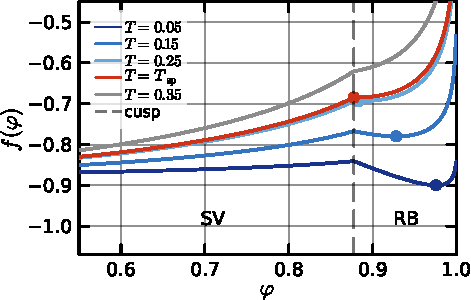
\includegraphics[width=0.45\textwidth]{panels_paper/cusp_illustration.pdf}
\caption{Leading-order free energy density $f(\varphi)$ at $\alpha=0.5$, $\Bnet=1$,
for several $T$. RB: retrieval basin; SV: saddle valley (where the spurious term
dominates); cusp at $\varphi\approx 0.877$ (dashed grey). Coloured dots mark the
RB minima; they disappear at the spinodal temperature
$T_{\rm sp}(\alpha, \Bnet) \approx 0.262$.}
\label{fig:cusp}
\end{figure}

The retrieval minimum is at
\begin{equation}
    \varphi_{\rm eq} = \tfrac{1}{2}(\sqrt{T^2+4} - T),
    \label{eq:phi_eq}
\end{equation}
so the spinodal condition $\varphi_{\rm eq} = \varphi_c(\alpha, \Bnet)$ yields
\begin{equation}
    T_{\mathrm{sp}}(\alpha, \Bnet) \;=\; \frac{\Bnet^2 - (\alpha + \gmax(\Bnet))^2}
              {\Bnet\,(\alpha + \gmax(\Bnet))}\,.    
    \label{eq:spinodal}
\end{equation}
For $T < T_{\mathrm{sp}}(\alpha, \Bnet)$ the retrieval minimum exists. It is
thermodynamically stable when it is the global minimum of $f$ and metastable when
the saddle-valley minimum is deeper. At equilibrium the deeper basin carries the
larger weight, with the ratio between the two basins set by their depth difference;
at finite $T$ and finite $N$ both basins can carry significant mass. The chain
escapes the retrieval basin to the saddle valley by a Kramers process at the same
rate $\sim \e^{-N \Delta f / T}$ in both regimes, with $\Delta f$ the per-spin
barrier from the basin minimum to the cusp; what differs is the return rate. A
Monte Carlo ensemble initialised in the basin contains both populations at finite
budget, in proportions set by the budget over the Kramers escape time. As
$T \to 0$ the escape rate vanishes, so retrieval is retained whenever the basin
exists.

\citet{ramsauer2021hopfield} bound the spurious sum by $M$ times its largest term,
\begin{equation}
S_{\rm spur} \le M\,\e^{-\Bnet N(1-\varphi_{\max})} = \e^{N(\alpha - \Bnet(1-\varphi_{\max}))},
\label{eq:ramsauer_bound}
\end{equation}
which exceeds the retrieval term once $\varphi_{\max} > 1 - \alpha/\Bnet$. The highest
alignment present is $\varphi_{\max} = \sqrt{1-\e^{-2\alpha}}$, so
\citeauthor{ramsauer2021hopfield}'s capacity solves
\begin{equation}
\sqrt{1-\e^{-2\alpha}} = 1 - \frac{\alpha}{\Bnet},
\label{eq:ramsauer_capacity}
\end{equation}
finite and $\Bnet$-dependent.

Fig.~\ref{fig:varphi} summarises the different approaches to the capacity. 
The red curve is the zero-temperature capacity from the saddle-point evaluation
of the spurious sum. It grows with $\Bnet$ and reproduces the exact spherical
threshold of \citet{lucibello2024exponential}.

The blue solid curve is the exact-density extreme $\varphi_{\max} = \sqrt{1-\e^{-2\alpha}}$
(no finite capacity); the blue dotted curve is its Gaussian approximation $\sqrt{2\alpha}$,
which gives the $\Bnet$-independent $\acGauss = 1/2$. The grey dashed line $1 - \alpha/\Bnet$
is the Ramsauer condition~\eqref{eq:ramsauer_capacity}; its intersection with the blue solid
curve gives the Ramsauer capacity, finite and $\Bnet$-dependent but below the red curve at
every $\Bnet$.

\begin{figure}[t]
\centering
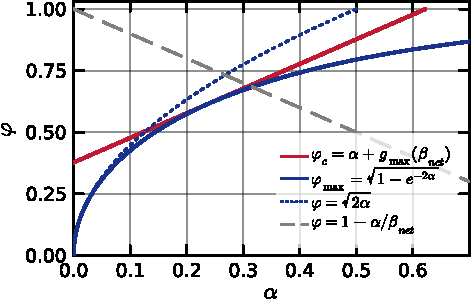
\includegraphics[width=0.45\textwidth]{panels_paper/cusp_vs_extreme.pdf}
\caption{Threshold curves at $\Bnet = 1$. Red straight line:
$\varphi_c(\alpha) = \alpha + g_{\max}(\Bnet)$, tangent to the blue solid curve at the
saddle $\varphi^*(\Bnet)$ (Appendix B). Blue solid:
$\varphi_{\max}(\alpha) = \sqrt{1-\e^{-2\alpha}}$, the exact-density extreme alignment.
Blue dotted: $\sqrt{2\alpha}$, its Gaussian approximation. Grey dashed:
$1 - \alpha/\Bnet$, the Ramsauer condition.}
\label{fig:varphi}
\end{figure}

The red line is tangent to the blue solid curve at every $\Bnet$; as $\Bnet$ varies,
the tangency point sweeps the entire blue solid curve. This follows from the
Legendre conjugacy between $g_{\max}(\Bnet)$ and $\varphi_{\max}(\alpha)$, derived in
Appendix B.
The geometric consequence is that the cusp $\varphi_c(\alpha, \Bnet)$ lies above the
maximum alignment $\varphi_{\max}(\alpha)$ at every $\alpha$: no individual spurious
pattern enters the retrieval basin $\varphi > \varphi_c$. Retrieval loss is therefore
\textit{collective}, driven by the bulk saddle of the spurious sum and not by any
single spurious pattern reaching the target. In the terminology of
\citet{lucibello2024exponential}, the retrieval boundary lies in the
\textit{uncondensed} phase of the auxiliary REM, where exponentially many patterns
dominate the noise sum, as opposed to the \textit{condensed} phase where a single
pattern dominates.

\section{Monte Carlo schemes}


\section{Results}


\section{Discussion}





% \section{Acknowledgments}


\bibliography{aaai2026}

\appendix

\section{Appendix A: Derivation of the prefactor in the spurious sum}

The integral~\eqref{eq:spur_integral} evaluates in closed form. Substituting
$\varphi = \cos\theta$ maps the spherical density onto the kernel of the integral
representation of the modified Bessel function
$I_\nu(z)$~\citep[8.431.3]{gradshteyn2015}; at $\nu = N/2 - 1$, $z = \Bnet N$,
this gives for $N > 1$
\begin{equation}
S_{\rm spur} = M \Gamma\Big(\tfrac{N}{2}\Big)\left(\frac{2}{\Bnet N}\right)^{\!N/2-1}\!\!\e^{-\Bnet N}\,I_{N/2-1}(\Bnet N).
\label{eq:spurious_exact}
\end{equation}
The right-hand side is the disorder expectation of the sum~\eqref{eq:spur_sum}. The
relative fluctuations of $S_{\rm spur}$ around this expectation are
$\sim \e^{N[\delta(\Bnet) - \alpha]/2}$ with
$\delta(\Bnet) = g_{\max}(2\Bnet) - 2\,g_{\max}(\Bnet) > 0$; they are exponentially
small in $N$ when $\alpha > \delta(\Bnet)$. At $\Bnet = 1$, $\delta \approx 0.334$,
well below the retrieval boundary $\alpha_c \approx 0.623$, so the
saddle~\eqref{eq:spurious_saddle} captures the typical $S_{\rm spur}$.


The Debye uniform asymptotic of the modified Bessel function~\citep[10.41.3]{olver2010nist}
gives the prefactor of~\eqref{eq:spurious_saddle}. Keeping the leading ($k = 0$) term of
the asymptotic series,
\begin{equation}
I_\nu(\nu z') \sim \frac{\e^{\nu\eta(z')}}{(2\pi\nu)^{1/2}(1+{z'}^2)^{1/4}},
\end{equation}
where $z' = 2\Bnet N/(N-2)$ and
\begin{equation}
    \eta(z') = \sqrt{1+{z'}^2} + \ln\frac{z'}{1+\sqrt{1+{z'}^2}}\,.
    \label{eq:bessel_debye}
\end{equation}  
$\eta(z')$ is expanded to $\mathcal{O}(N^{-1})$ because it is multiplied by
$\nu = N/2 - 1$ in the exponent:
\begin{equation}
    \eta(z') = \eta(2\Bnet) + \eta'(2\Bnet) \frac{4\Bnet}{N} + O(N^{-2})\,,
\end{equation}
where
\begin{align}
    \eta(2\Bnet)  &= 1 + 2\Bnet\varphi^* + \ln\varphi^*\,, \\
    \eta'(2\Bnet) &= \varphi^* + \frac{1}{2\Bnet}\,.
\end{align}
Then 
\begin{equation}
    \nu \eta(z') = \tfrac{N}{2} \eta(2\Bnet) - \ln\varphi^* + \mathcal{O}(1/N).
\end{equation}
The $\mathcal{O}(1)$ piece $-\ln\varphi^*$ in the exponent contributes a factor
$1/\varphi^*$ to the prefactor. Using Stirling's formula
\begin{equation}
    \Gamma(N/2) \sim \sqrt{4\pi/N}\,(N/2)^{N/2}\,\e^{-N/2}
\end{equation} 
and collecting all terms in~\eqref{eq:spurious_exact} to $\mathcal{O}(1)$ in the
exponent and to leading order in the prefactor reproduces the exponent
of~\eqref{eq:spurious_saddle} and gives the prefactor:
\begin{equation}
S_{\rm spur} \approx \frac{\e^{N[\alpha + g_{\max}(\Bnet) - \Bnet]}}{\sqrt{1-\varphi^{*4}}}
\label{eq:spurious_laplace}
\end{equation}
with $g_{\max}(\Bnet)$ given by \eqref{eq:saddle_value}.
At $\Bnet = 1$, $\varphi^* \approx 0.618$ and the prefactor is $\approx 1.082$.


\section{Appendix B: Legendre-conjugacy relation between the saddle value and the spherical extreme}

At fixed $\Bnet$, the cusp $\varphi_c(\alpha, \Bnet) = (\alpha + g_{\max}(\Bnet))/\Bnet$
is a line in $\alpha$ with slope $1/\Bnet$. As $\Bnet$ varies, this one-parameter
family of lines has the spherical extreme
$\varphi_{\max}(\alpha) = \sqrt{1-\e^{-2\alpha}}$ as its lower envelope, tangent at
the spherical saddle $\varphi^*(\Bnet)$.

The envelope condition $\partial_\Bnet \varphi_c|_\alpha = 0$ gives
\begin{equation}
\Bnet\, g'_{\max}(\Bnet) - g_{\max}(\Bnet) = \alpha.
\end{equation}
From $g_{\max}(\Bnet) = \tfrac12 \ln(1-\varphi^{*2}) + \Bnet\,\varphi^*$ and the
saddle equation $\Bnet\,\varphi^{*2} + \varphi^* - \Bnet = 0$, $g'_{\max}(\Bnet) = \varphi^*$,
so the tangency abscissa is
\begin{equation}
\alpha_0(\Bnet) = \Bnet\,\varphi^* - g_{\max}(\Bnet) = -\tfrac12 \ln(1-\varphi^{*2}).
\label{eq:alpha_tangent}
\end{equation}
At $\alpha = \alpha_0$ the line takes value $\varphi^*(\Bnet)$.
Squaring~\eqref{eq:alpha_tangent} gives $\varphi^{*2} = 1 - \e^{-2\alpha_0}$, so
$(\alpha_0, \varphi^*)$ lies on the spherical extreme. As $\Bnet$ sweeps
$(0, \infty)$, $\varphi^*$ sweeps $(0, 1)$, and the tangency point traces the full
curve.

The spherical extreme is concave ($\varphi_{\max}''(\alpha) < 0$), so each cusp
line lies above it except at tangency, and
\begin{equation}
\varphi_{\max}(\alpha) = \inf_{\Bnet > 0} \varphi_c(\alpha, \Bnet).
\end{equation}
$g_{\max}(\Bnet)$ and $-\tfrac12 \ln(1-\varphi^2)$ are Legendre conjugates.


\end{document}
